\begin{frame}{Grounding lines}
  \begin{columns}
    \begin{column}{0.45\textwidth}
      \centering
      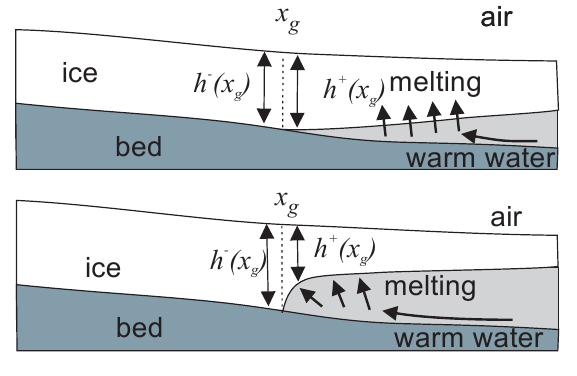
\includegraphics[width=\textwidth]{figures/GroundingLine/circulation} \\
      \vspace{-.5em}
      {\tiny Schoof 2007} \\
      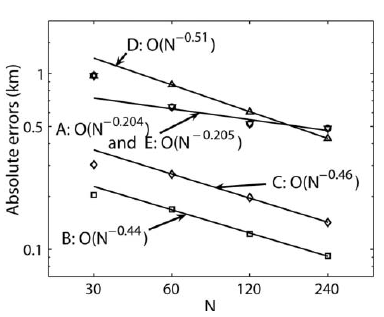
\includegraphics[width=\textwidth]{figures/GroundingLine/isothermal-Linfty} \\
      \vspace{-.5em}
      {\tiny Bueler et. al. 2005}
    \end{column}
    \begin{column}{0.55\textwidth}
      \begin{itemize}
      \item ocean circulation is very sensitive to grounding line
        geometry, feedback
      \item non-shallow physics applies in vicinity of grounding line
      \item current models are less than first-order accurate at margins
      \item extremely high resolution needed for qualitatively correct
        results on Eulerian meshes
      \end{itemize}
    \end{column}
  \end{columns}
\end{frame}
